 % mainfile: ../../../../master.tex
\subsection{Migrate Zicheng's code}
\label{task:20240314_aosp}

\subsubsection{Customize AOSP 14}

\begin{longtable}{p{.20\linewidth}p{.37\linewidth}p{.37\linewidth}} 
\toprule
file & Customized AOSP13 & Changes in 14 \\
\midrule
\endhead

\path{java_vm_ext.cc}
& Modify \texttt{FindSymbol}.
& No changes for \texttt{FindSymbol}.
\\

\path{art_method.h}
& Modify \texttt{UpdateCounter} declaration.
& No changes for \texttt{FindSymbol}.
\\

\path{art_method-inl.h}
& Modify \texttt{UpdateCounter} definition (added unused variable declarations)
& No changes for \texttt{FindSymbol}.
\\

\path{art_method.cc}
& Modify \texttt{Invoke}, and \texttt{PrettyMethod}.
& No changes for \texttt{Invoke}.
\\

\path{app_info.h}
& Add \texttt{GetPackageName} public declaration.
& No related changes.
\\

\path{app_info.cc}
& Add \texttt{GetPackageName} definition.
& No related changes.
\\

\path{runtime.h}
& Add \texttt{NativeLibFunc} struct, public declaration for a lot of functions and variables.
& No related changes.
\\

\midrule
\caption{Customizing AOSP 14} 
\label{tab:customizingaosp14}
\end{longtable}

\subsubsection{Scripts}

Script to run the emulator and log console outputs:
\begin{lstlisting}[language=bash]
emulator & 
adb wait-for-device
A=$(adb shell getprop sys.boot_completed | tr -d '\r')

while [ "$A" != "1" ]; do
        sleep 1
        A=$(adb shell getprop sys.boot_completed | tr -d '\r')
done

adb root
echo "[WEIMINN] Enabling logging"
adb shell setprop debug.ld.all dlerror,dlopen
rm -f logcat.txt 
echo "[WEIMINN] Logging with Logcat to logcat.txt"
adb logcat >> logcat.txt
\end{lstlisting}

Script to kill running emulator process:
\begin{lstlisting}[language=bash]
adb devices | grep emulator | cut -f1 | while read line; do adb -s $line emu kill; done
\end{lstlisting}

Script for finding a string:
\begin{lstlisting}[language=bash]
cd /home/weiminn/Documents/aosp14/

clear

find \
    ./frameworks/ ./art/ ./bionic/ \
    \( -iname '*.java' -o -iname '*.cpp' -o -iname '*.cc' -o -iname '*.hpp' -o -iname '*.h' -o -iname '*.S' \) \
    -a ! -iname '*test*' -a ! -iname '*out*' \
    | xargs grep --color -sin 'invoke'
\end{lstlisting}

Comment to annotate added code:
\begin{lstlisting}[language=bash]
/////////////////////// DYNDROID-START ///////////////////////
/////////////////////// DYNDROID-END ///////////////////////
\end{lstlisting}

\subsubsection{Problems}

Faced problem in \path{runtime.h} after copying in
\begin{lstlisting}[language=c++]
void setLoadingSchema(bool loading, std::string s){
    ALOGW("[Zicheng_Content_Provider] runtime.h setLoadingSchema() package:%s, %s", s.c_str(), loading ? "true" : "false");
    loading_schema_ = loading;
}

void setLoadedSchema(bool loaded, std::string s){
    ALOGW("[Zicheng_Content_Provider] runtime.h setLoadedSchema() package:%s", s.c_str());
    loaded_schema_ = loaded;
}

void setShouldReadSchema(bool should, std::string s){
    ALOGW("[Zicheng_Content_Provider] runtime.h setShouldReadSchema() package:%s, %s", s.c_str(), should ? "true" : "false");
    should_read_schema_ = should;
}
\end{lstlisting}
because there is no definition for \texttt{ALOGW}, so I put \texttt{\#include "utils/Log.h"} at the top of \path{runtime.h}, and it worked!

Need to edit and compile \path{runtime.h} and \path{runtime.cc} after editing \path{art_method.cc}, as it calls \path{Runtime::MYmatch_target_method}.

Changes to \texttt{void Instrumentation::InitializeMethodsCode} by both DynDroid and AOSP 14.

What does \texttt{.clang-format} mean?

% 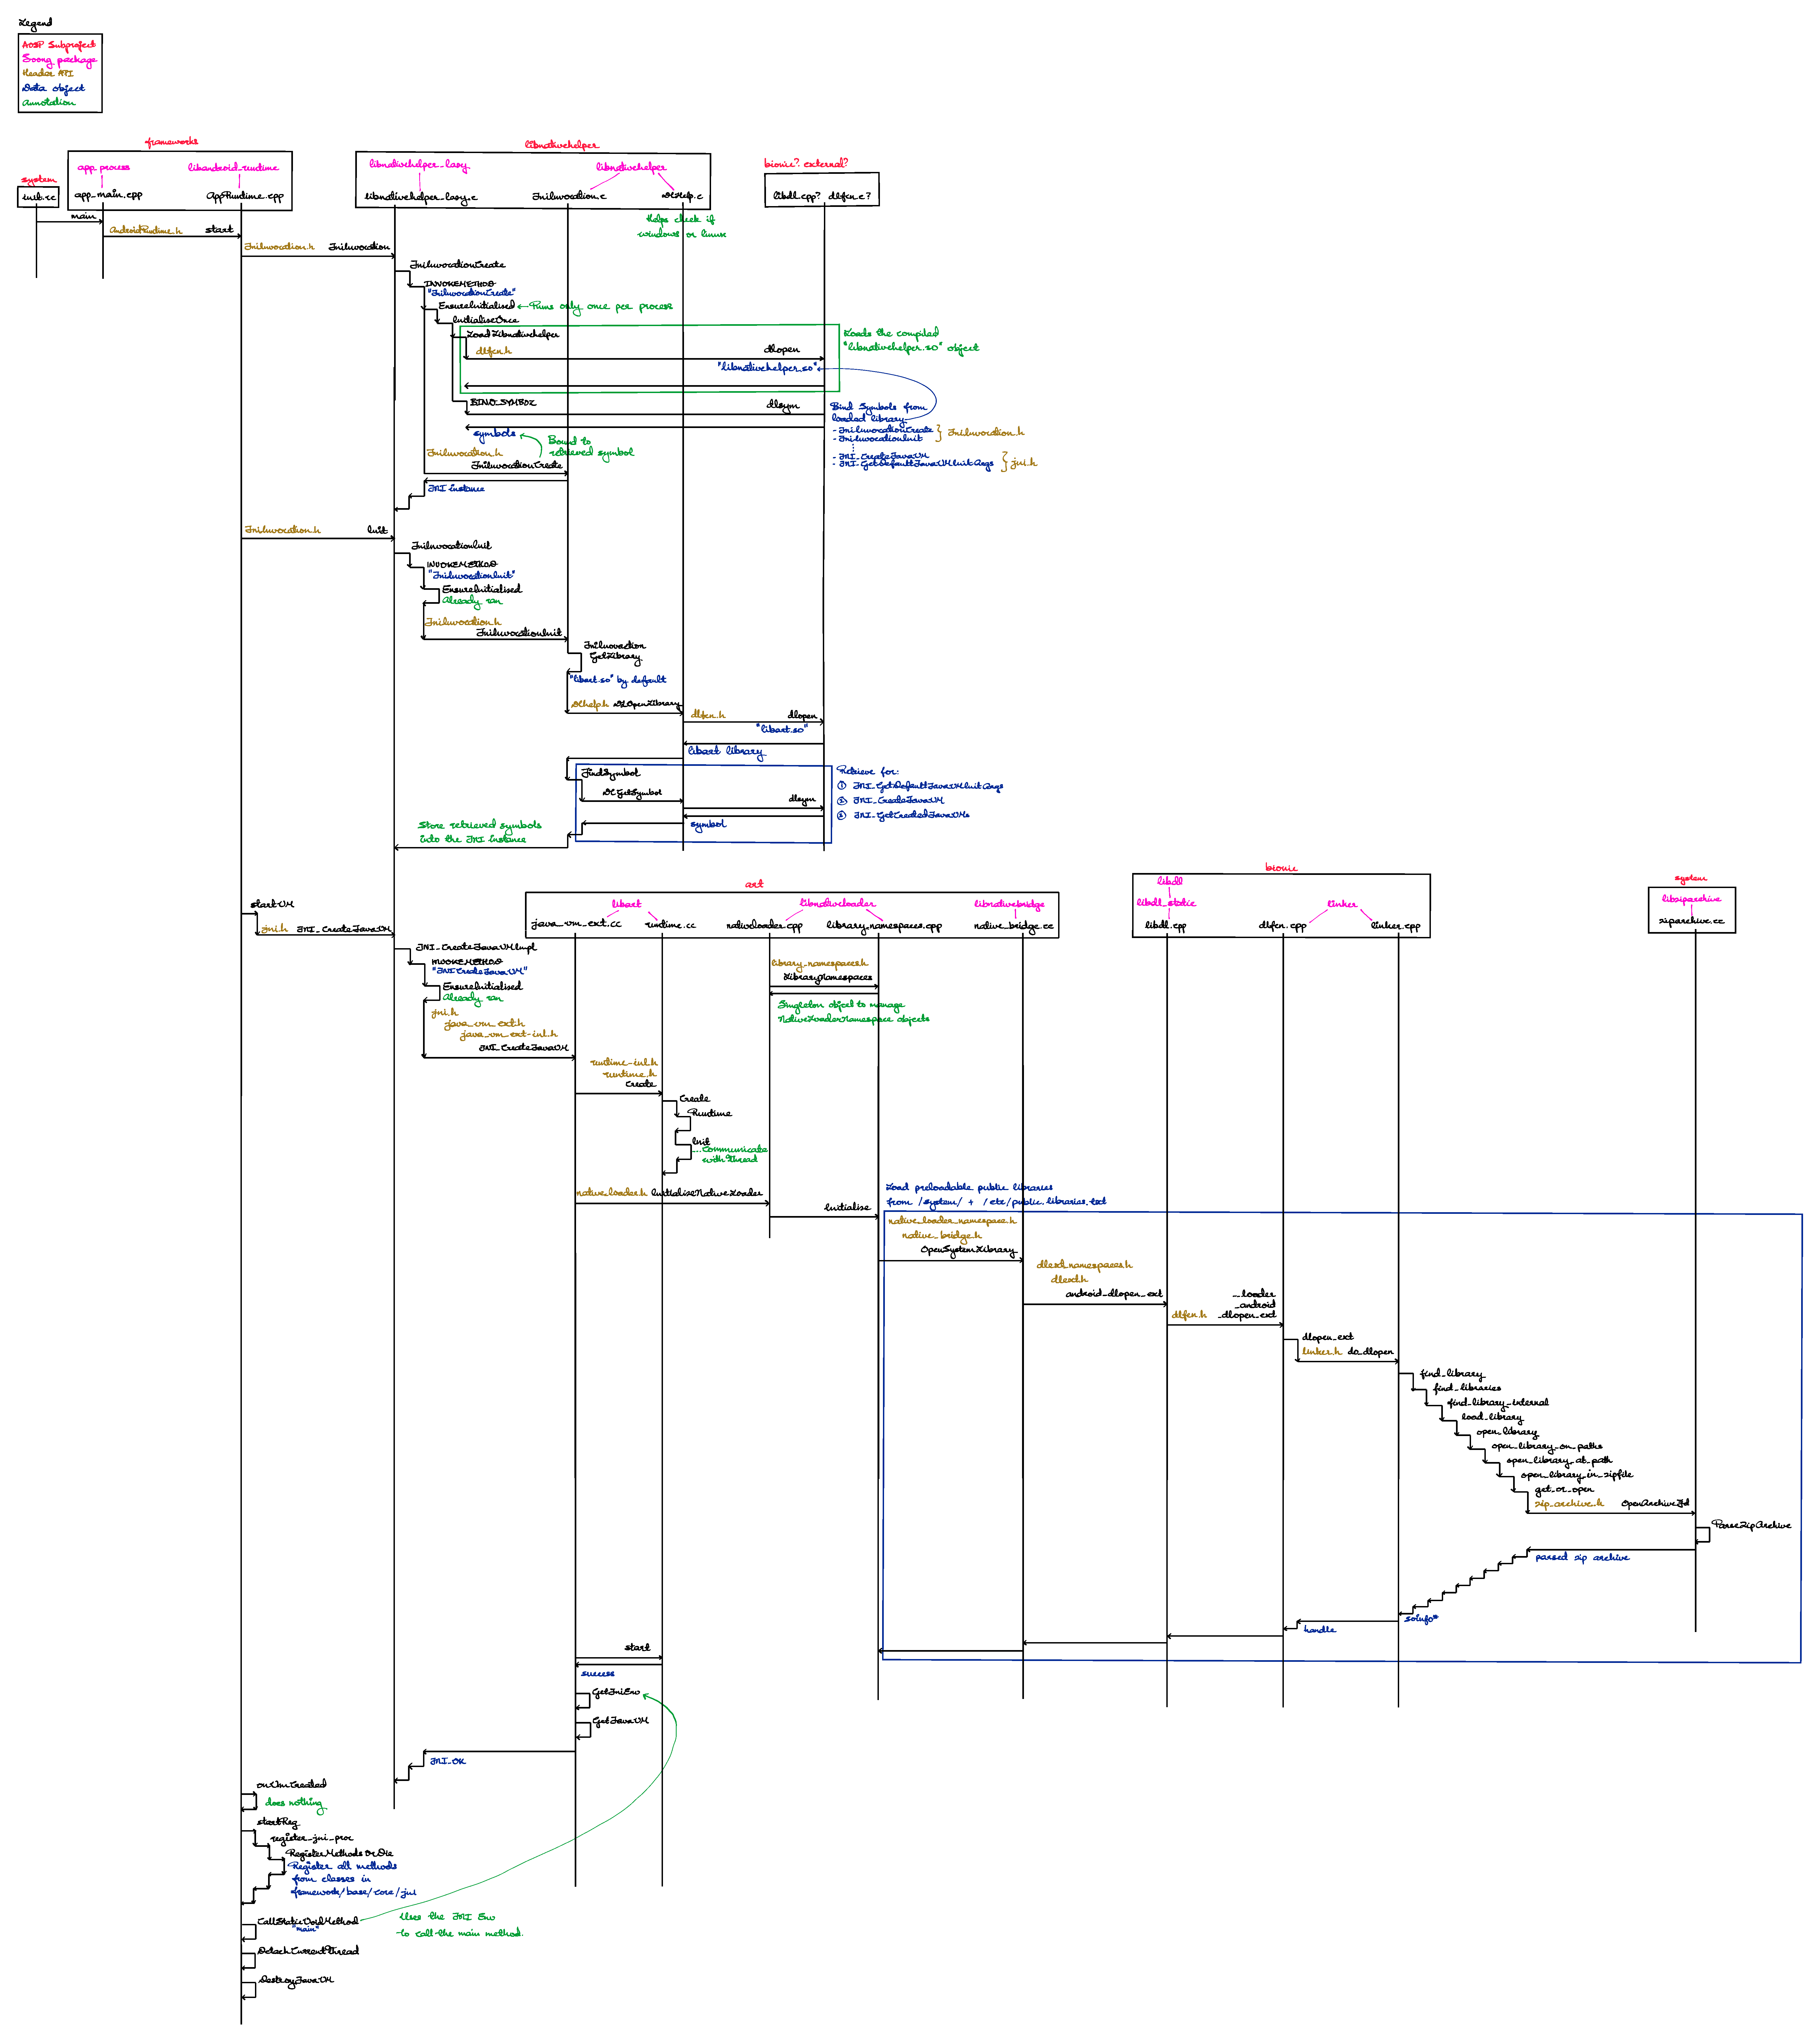
\includepdf[pages=-, scale=.95,pagecommand={}]{entries/2024/01/01/art.pdf}

% \begin{itemize}
% \item \textbf{Domain.} The context of the process that is acting upon something.
% \item \textbf{Type.} The context of the resource on which the process is acting.
% \item \textbf{Class.} The object class of the resource (e.g. \textit{file} or \textit{socket}).
% \item \textbf{Permissions.} The permissions that are allowed given the \textit{domain}, \textit{type} and \textit{class}.
% \end{itemize}

% SELinux rule syntax:


% \subsubsection{Decoding Permission Denial Message}

% Message:
% \begin{lstlisting}
% type=AVC msg=audit(1363289005.532:184): avc:  denied  { read } for  pid=29199 comm="Trace" 
% name="online" dev="sysfs" ino=30 scontext=staff_u:staff_r:googletalk_plugin_t 
% tcontext=system_u:object_r:sysfs_t tclass=file
% \end{lstlisting}

% \begin{longtable}{p{.15\linewidth}p{.15\linewidth}p{.65\linewidth}} 
% \toprule
% Log part & Name & Description \\
% \midrule
% \endhead

% \texttt{type=AVC}
% &Log type
% &Only in the \texttt{audit.log} file; it informs the user what kind of audit log type this is. 
% \\

% \texttt{msg=audit(1363289005.532:184)}
% &Timestamp
% &Timestamp in seconds since epoch, meaning the number of seconds since January 1st, 1970. You can convert this to a more human readable format using date -d @ followed by the number, like so: \texttt{date -d @1363292159.532}.
% \\

% \texttt{avc:}
% &Log type (again)
% &
% \\

% \texttt{ino=30}
% &inode number
% &The inode number of the target file. In this case, since we know it is on the \texttt{sysfs} file system, we can look for this file using: \texttt{find /sys -xdev -inum 30}
% \\

% \texttt{scontent=staff\_u:staff\_r:googletalk\_plugin\_t}
% &Source context
% &The security context of the process (the domain)
% \\

% \texttt{tcontext=system\_u:object\_r:sysfs\_t}
% &Target context
% &The security context of the target resource (in this case the file)
% \\

% \texttt{tclass=file}
% &Target class
% &The class of the target.
% \\

% \midrule
% \caption{Permission Denied Syntax} 
% \label{tab:permissiondeniedsyntax}
% \end{longtable}


% \subsubsection{SELinux Architecture}

% SELinux consists of four main components: object managers (OM), access vector cache (AVC), security server, and security policy as show below:
% \begin{figure}[H]
%     \centering
%     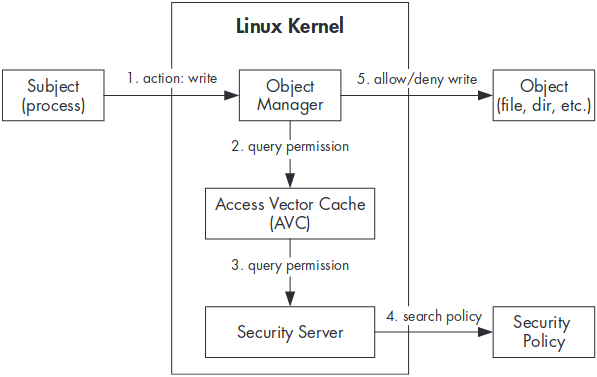
\includegraphics[width=.85\linewidth]{entries/2023/12/10/selinux.png}
%     \caption{SELinux Components}
%     \label{fig:selinux}
% \end{figure}
